% =============================================================================
% Template dissertation using the qdissertation class
% =============================================================================
% This file is the main entry point. Build: make (uses latexmk; see Makefile).
% Default engine: lualatex. To use another: make ENGINE=pdf or make ENGINE=xe.
%
% SPDX-FileCopyrightText: 2026 Frank Langbein <frank@langbein.org>
% SPDX-License-Identifier: LPPL-1.3c
% SPDX-License-Identifier: CC-BY-SA-4.0
%
% This template and other .tex/.bib files in this directory are part of the
% same work and may be distributed and/or modified under the LaTeX Project
% Public License (LPPL), version 1.3c. See LICENSE file.
%
% -----------------------------------------------------------------------------
% Overview (qdissertation class)
% -----------------------------------------------------------------------------
% The class is a wrapper around the standard book class. Layout: A4, 12pt,
% 3cm margins; single line spacing; ragged-right; main text 12pt, footnotes and
% captions at least 11pt; preliminary pages in roman numerals, then Arabic
% for main matter. Chapter style: top bar in header, ``Chapter N'' or
% ``Appendix A'' in header; number/letter and title on first line of chapter.
%
% -----------------------------------------------------------------------------
% Report structure
% -----------------------------------------------------------------------------
% Main body: Introduction, Background, Methodology (or ``Specification, Design
% and Implementation'' / ``Approach''), Results and Evaluation, Conclusions and
% Future Work, Reflection on Learning. Chapter~3 can be adapted or split; not all
% sections apply to every project (system design, research, AI/ML). See each
% chapter file for details and alternatives.
%
% Suggested sections at a glance (omit/rename as needed):
%   1 Introduction:    Motivation and context; Aims and objectives; Contributions;
%                      Dissertation structure. Optional: Scope, Terminology.
%   2 Background:      Context; Related work (or Literature review); Problem statement.
%                      Optional: Theory and concepts; Stakeholders and constraints.
%   3 Methodology:     Depends on project type. System design: Specification, System
%                      design, Implementation. Research: Research design, Literature
%                      and evidence, Approach and solution, Implementation. AI/ML:
%                      Specification, Datasets, AI/ML models, System design, Implementation.
%                      Optional: Ethical considerations; Summary.
%   4 Results:         Setup (or Experimental setup); Results; Discussion; Limitations.
%                      Optional: Ablation studies; Comparison with baselines.
%   5 Conclusions:     Conclusions; Future work.
%   6 Reflection:      Critical narrative; Analysis and application; Implications
%                      for future practice. (Omit chapter if not required.)
%
% -----------------------------------------------------------------------------
% Variations (degree, structure)
% -----------------------------------------------------------------------------
% Select your degree via \degree below; commented alternatives shown for
% BSc, MSc.
%
% -----------------------------------------------------------------------------
% Class options
% -----------------------------------------------------------------------------
% Font: sans (default), serif, or hacker;
%   serif = serif text and math; hacker = typewriter/monospace open-source font throughout.
% Layout: oneside (default) or twoside.
% Citation: numeric (default) = plainnat, [1], [1,2]; harvard = agsm, (Author, 2000).
% Alignment: raggedright (default) = ragged-right; justified = fully justified text.
% Line spacing: single (default); onehalfspacing; or linespread115/linespread12
%   for institutions allowing 1.0--1.3.
% Paragraph style: parskip (default) = space between paragraphs, no first-line indent;
%   parindent = traditional first-line indent, minimal parskip.
% Optional typography:
%   fullwidth  = enable \begin{fullwidth}...\end{fullwidth} and fullwidthfigure/
%                fullwidthtable environments that extend into the margin (requires
%                changepage or chngpage).
%   italic = chapter, section, subsection and captions in italic (default: bold/roman).
% Engine: pdfTeX vs XeLaTeX/LuaLaTeX is detected for font setup.
%
% Defaults (no option): link colour DarkBlue, cite/URL colour DarkGreen; tight list
% margins; quote, quotation, and verse in smaller type with indents;
% \epigraph{quote}{source} for chapter/section-opening quotes.
% See Section~\ref{sec:ch1-reference} in Chapter~1 for examples of \newthought,
% fullwidth, fullwidthfigure, quote, and epigraph.
%
% -----------------------------------------------------------------------------
% Metadata and title page
% -----------------------------------------------------------------------------
% \title, \author, \degree, \university, \date drive the generated title page.
%
% -----------------------------------------------------------------------------
% License and copyright (SPDX)
% -----------------------------------------------------------------------------
% \copyrightholder defaults to \author; \licenseyear defaults to current year.
% When \license is set: (1) a copyright page is inserted after the abstract;
% (2) a License chapter is inserted just before the bibliography.
% If qdissertation-licenses.tex is present, the class loads it for full
% license text; otherwise name + URL only.
%
% -----------------------------------------------------------------------------
% Float placement (figures, tables, algorithms)
% -----------------------------------------------------------------------------
% Placement letters: h = here, t = top, b = bottom, p = float page. E.g.\@
% [htbp], [t], [!t]. Use [H] (float pkg) sparingly. The class relaxes float
% parameters so more floats fit per page.
%
% -----------------------------------------------------------------------------
% Headings: use title case for chapter titles (capitalise major words; keep
% articles, conjunctions, and short prepositions lowercase unless first/last
% word). Use sentence case for sections, subsections, and below (only the
% first letter and proper nouns capitalised). Or adjust as preferred, but keep
% it consistent.
%
% -----------------------------------------------------------------------------
% LaTeX formatting: \citep/\citet (not \cite); ~ before \citep/\citet after a word;
% \@ after abbreviation; ~ for non-breaking (Fig.~1); -- en-dash, --- em-dash.
%
% -----------------------------------------------------------------------------
% Reviewer comments: %ID (e.g.\@ %F) at line start, space after ID. Include
% comments directly in the text and discussions or questions can be included
% as comments afterwards. Generally, these comments should be inserted closely
% after the sentence or element it refers to. Delete the commetns when
% addressed; do not keep ``for checking''. Edits can be easier found via git
% diffs. Find comments with: grep -r '^%[A-Za-z] ' *.tex */*.tex
%
% -----------------------------------------------------------------------------
% Footnotes: prefer putting short asides in parentheses in the main text. Use
% footnotes only sparingly when they add value (e.g.\@ translations, optional
% clarifications that would interrupt the flow).
%
% -----------------------------------------------------------------------------
% Word count: run ``make wordcount'' (texcount -inc; per-file and total with
% caption words shown separately so you can apply your institution's rules).
% Word limits typically apply to main body only; exclude front matter, captions,
% appendices. Confirm your institution's word limits and structure before submission.
%
% -----------------------------------------------------------------------------
% Submission: ensure PDF has embedded fonts (pdflatex does this by default),
% and is compatible with your institution's requirements (e.g. no encryption, be
% careful with obfuscation).
% =============================================================================
\documentclass[sans,oneside,numeric,raggedright,fullwidth]{qdissertation}

% -----------------------------------------------------------------------------
% Optional: use a different acronyms file
% -----------------------------------------------------------------------------
%\renewcommand{\qdissertationacronymfile}{my-acronyms.tex}

% -----------------------------------------------------------------------------
% Useful packages for dissertation writing
% -----------------------------------------------------------------------------

% Tables
\usepackage{tabularray}      % Flexible column types, rules, longtblr for multi-page tables
\usepackage{booktabs}        % Alternative (traditional): \toprule, \midrule, \bottomrule
\usepackage{longtable}       % Tables that span multiple pages (or use tabularray longtblr)
%\usepackage{multirow}        % Span multiple rows in tables
%\usepackage{multicol}        % Multiple columns in text/tables
%\usepackage{colortbl}        % Coloured rows/cells in tables

% Math, symbols, related
\usepackage{mathtools}       % Extensions to amsmath (matrix envs, \DeclarePairedDelimiter)
\usepackage{pifont}          % Dingbat symbols, e.g. \ding{51}, \ding{43}
\usepackage{siunitx}         % Units and numbers: \SI{3}{m/s}, \num{1000}
\usepackage{relsize}         % \textlarger, \textsmaller for relative font sizing
\usepackage[version=4]{mhchem} % Chemical formulae: \ce{H2O}, \ce{CO2}, \ce{^1H-NMR}

% Floats
\usepackage{float}           % [H] = here definitely
\usepackage{stfloats}        % Improved placement for bottom floats
\usepackage{subcaption}      % Subfigures with (a), (b) and per-subfigure captions
\usepackage{rotating}        % \begin{sidewaystable}, \begin{sidewaysfigure} for wide content

% Algorithms
\usepackage{algorithm}       % Numbered algorithm floats and List of Algorithms
\usepackage[noend]{algpseudocode}

% Other useful packages
\usepackage{lipsum}          % Placeholder text: \lipsum[n], \lipsum[1-5], etc.
\usepackage{enumitem}        % Customise list labels, spacing
\usepackage{verbatim}        % \begin{verbatim} ... \end{verbatim} for code
\usepackage{afterpage}       % \afterpage{\clearpage} to clear after current page

\usepackage{multirow}

\setcounter{secnumdepth}{3} % Allow numbering down to subsubsections
\setcounter{tocdepth}{3}    % Allow subsubsections in the Table of Contents

% -----------------------------------------------------------------------------
% Dissertation metadata
% -----------------------------------------------------------------------------

% \title{
%   Hierarchical Metric-Semantic SLAM Methods for Architectural Mapping
%   
\includegraphics[width=0.4\textwidth]{figures/Cardiff-logo.png}\\[1cm]
% }

%\title{Hierarchical Metric-Semantic SLAM Methods for Architectural Mapping}
%\author{Jasper Wilkes}

\title{Hierarchical Metric-Semantic SLAM Methods for Architectural Mapping}

\author{
    Jasper Wilkes \\[1cm] 
    
\includegraphics[width=0.4\textwidth]{figures/Cardiff-logo.png}
}

% Degree
\degree{BSc Computer Science}
% \degree{MSc Advanced Computer Science}
\university{Cardiff University}
\date{February 2026}

% License and copyright following SPDX. (optional; comment out if not needed).
% Needs qdissertation-licenses.tex for license text in the License chapter.
\license{CC-BY-SA-4.0}
\copyrightholder{Jasper Wilkes}
\licenseyear{2026}

%add glossaries
\makeglossaries

\begin{document}

\frontmatter

% \maketitle{...} produces: title page, (copyright page if \license set), abstract,
% then frontlists: TOC, List of Figures, List of Tables, List of Algorithms,
% List of Acronyms (if acronyms.tex defines \newacronym).
% Add \dedication{...} and \makededication separately if desired.

% This is the abstract: a short, self-contained summary of the dissertation.
% It should state the problem, methods, and main results so that a reader
% can understand the scope without reading the full document. Replace with
% your own abstract.
\maketitle{%
  % Abstract: typically 200--300 words. State problem, methods, and main results.  
  \gls{slam} is the fundamental robotics 
  problem of estimating both the pose of a mobile robot and a map of its surroundings.
  Recent advancements addressing the \gls{slam} problem use a graph-based representation of a 
  scene that integrates metric (occupancy) and semantic (classes) estimates, along with 
  hierarchical relationships connecting different aspects of the scene (e.g. an object belongs to a room). 
  This representation, known as a \gls{dsg}, encompasses actionable 
  information that aids in robot planning and decision-making, but also in supporting 
  architecture-related tasks such as renovation, inventory and remote building visualisation.
  
  This project focuses on deploying and evaluating three state-of-the-art \gls{dsg} methods in a 
  simulated environment: S-Graphs+ \cite{s_graphs_plus}, Hydra \cite{hydra} and Clio \cite{clio}. The best performing method 
  was then used to process real world data and create a \gls{dsg} of the \gls{hccr} laboratory. Each method uses a different approach to creating the \gls{dsg}: 
  S-Graphs+ is geometry based, Hydra adopts a Spatial approach while Clio uses a Task-Driven approach.

  The evaluation revealed that S-Graphs+ struggled in cluttered environments, as objects like desks
  often prevented the method from fully identifying wall planes, leading to incorrect classification and over-segmentation of rooms.
  Clio excelled at segmenting and labelling regions correctly with a recall of 0.93, however over-segmented rooms with 0.45 Precision. It also correctly labelled all detected regions, however struggled at object detection.
  A critical failure of Clio was it needing 0.25x playback speed to avoid missing frames or crashing. This failed the mandatory requirement of real-time processing, which eliminated it as a candidate for real world deployment.

  Hydra stood out as the best performing method. It showed high room Precision 0.90, however was conservative with Recall 0.43. It exhibited strong object detection skills (F1: 0.62), and demonstrated consistent object localisation across runs (Avg 0.16m).
  Semantic labelling struggled with Weighted Average F1 of 0.35, with the method often labelling computers and monitors as "Thing", due to a label space mismatch.

  Hydra was consequently used to create a \gls{dsg} of the \gls{hccr} laboratory using real world data. The resulting \gls{dsg} correctly identified one room and correctly identified key objects within the lab like storage, wall decorations and workstation equipment.

  Overall, Hydra has the potential to be useful for the architectural industry. The method's strong object detection could be used for inventory management tasks, while the high-precision room segmentation could be valuable for remote building visualisation. However, the method's conservative room segmentation and closed-set semantic limitations would need to be addressed for it to be more widely applicable.
}

% -----------------------------------------------------------------------------
% Optional front-matter chapters (unnumbered)
% -----------------------------------------------------------------------------

% Replace with your dedication (one or two lines); optional.
\dedication{%
  To my family.%
}

\chapter{Acknowledgements}
% Replace with your acknowledgements. Here you can also acknowledge any contributions from other
% parties to the work.
I thank my supervisors and colleagues for their support.

%\chapter{Declaration}
% Replace with your declaration (e.g. that the work is your own, and any
% required statements on collaboration, publications, or word count).
% Often this is submitted in separate forms or not needed, and does not
% have to be here.
%This dissertation is the result of my own work. Where reference is made to other work, this is indicated in the text.

%\chapter{Publications, data and code}
\chapter{Data and Code}
% List publications, if available or maybe planned, and state where data and code produced for this
% dissertation are available. Note, you usually must submit any sources and simlar you ahve
% written with your dissertation.
% Replace with your own entries; you can use \citep{key} for publications.

%\section{Publications}
% Papers (and optionally other outputs) that form part of or arise from this thesis.
% These can also be discussed in the introduction (what has been published or is planned).
%\begin{enumerate}
%  \item Author. Title. \textit{Journal}, volume, pages, year.~\citep{example-paper}
%\end{enumerate}

\section{Data}
% Datasets produced in this work and where they are available (repository, DOI, or ``on request'').
Data supporting this dissertation are available from [repository/DOI or ``available on request'']. Replace with your statement.

\section{Code}
% Software or code produced in this work and where it is available (repository, DOI, etc.).
Code produced for this dissertation is available at https://github.com/Jabasco291/Final-Year-Project.

\section{AI Tool Use and Acknowledgement}\label{ai-use}

To accelerate project infrastructure setup, two deployment infrastructure components were developed with assistance from Claude (Anthropic) \cite{Claude2024}, a ROS2 bag creation script (svo2\_to\_rosbag.py) and a custom odometry-TF republishing node (name of node). This approach was justified to accelerate the setup of project-specific infrastructure which allowed more focus towards evaluation of the best-performing method. All AI-assisted code was manually reviewed and validated before use to ensure correct logic and implementation.

\mainmatter

% -----------------------------------------------------------------------------
% Main chapters (suggested structure in each chapter file; adjust to your project)
% -----------------------------------------------------------------------------
\chapter{Introduction}\label{ch1}
% =============================================================================
% CHAPTER 1: Introduction
% =============================================================================
% SPDX-FileCopyrightText: 2026 Frank Langbein <frank@langbein.org>
% SPDX-License-Identifier: LPPL-1.3c
%
% Suggested sections: Motivation and context; Aims and objectives; Contributions;
% Dissertation structure (roadmap). Optional: Scope (boundaries of the work),
% Terminology or key terms. Start with a short chapter intro (no \section) before
% the first section. This file also demonstrates template features; see
% Section~\ref{sec:ch1-reference}. Remove that section for your own report.
% =============================================================================

% -----------------------------------------------------------------------------
% Chapter intro (no section): one short paragraph before the first \section
% -----------------------------------------------------------------------------
This chapter introduces the project's motivation and context for the work, the aims and objectives, the main contributions, and the structure of the remaining chapters. The following sections expand on each of these.

% -----------------------------------------------------------------------------
% Motivation and context (typical first section)
% -----------------------------------------------------------------------------
% Use \section, \subsection, \label{key}. Refer with \ref{key} or \autoref{key}.

\section{Motivation and context}\label{sec:motivation}

% \newthought{This template illustrates} the structure and style of a dissertation using the Qyber dissertation class. As in a real introduction, you would state the problem domain, why it matters, and how your work fits. Acronyms use the long-short style: first use gives the full form (e.g.\@ \gls{uk}); later use \acrshort{api} or \acrlong{api} when you need only short or long.

% As shown in previous work~\citep{example-paper}, we follow standard practice.
% %F Clarify whether this applies to all cases.
% \citet{example-book} provide a longer treatment; multiple citations: \citep{example-paper,example-conf}. You can link to other chapters (e.g.\@ Chapter~\ref{ch2}, Section~\ref{sec:objectives}) and to figures (Fig.~\ref{fig:demo}). The class provides \url{https://example.com} and \href{https://example.com}{link text} for URLs and hyperlinks.

\gls{slam} is the fundamental problem in robotics of an online robot making a map of its surroundings (mapping), whilst simultaneously tracking its own position (localisation). This enables actions such as path planning. This presents a chicken and egg problem, you need the map to calculate position, yet need the position to build the map.

Classical approaches to the \gls{slam} problem represent the environment using only metric terms such as occupancy grids, which captures the raw geometry without any structural meaning. Whilst this is enough for basic navigation, increasingly advanced robotics require a more structured understanding of the scene in order to execute higher-level functions. This is particularly apparent in architecture contexts, where tasks like inventorying or remote visualisation require an understanding of spatial structure.

As acknowledged in \cite{topologic}, current methods for building documentation rely on  inferred geometry and do not explicitly represent spatial connectivity or enclosure. This limits real-world applications such as inventorying, which needs room-level semantic partitioning to associate objects with spaces. Existing solutions such as Topologic \cite{Jabi2025} acknowledges this problem, however it still depends on initial human input for the topology. This motivates an automated system for scanning a real environment to create a topological spatial model, which can then assist in the applications discussed above.

Recent advancements in \gls{slam} research use a graph-based representation of the scene that integrates metric(occupancy) and semantic (classes) estimates, along with hierarchical relationships connecting different aspects of the scene. For example, an object belongs to a room. This approach, known as a \gls{dsg}, enables it to have a broader range of higher-level tasks, such as responding to natural language commands like ‘pickup the red pen’, or architecture-related tasks mentioned above.

Different \gls{dsg} methods use different approaches to how the scene is processed. This means they differ in how the scene is constructed and labelled. This proposes 3 core research questions: Which achieves the best accuracy, which is the most practical for deployment, and which creates the richest semantic understanding? This dissertation addresses these questions through a side-by-side evaluation of 3 state-of-the-art methods, resulting in deploying the best-performing method on real-world data.

% -----------------------------------------------------------------------------
% Aims and objectives (typical second section)
% -----------------------------------------------------------------------------
% Use \citep{} (parenthetical) or \citet{} (narrative), not \cite.

\section{Aims and objectives}\label{sec:objectives}

%State the aim of your project and break it down into objectives. The following is a placeholder list (enumitem package: custom labels).
The main aim of this project was to compare how 3 state-of-the-art methods perform according to different metrics, which would allow a best-performing to be selected to create a \gls{dsg} of the \gls{hccr} laboratory.
The project was broken down into 4 clear objectives:

\begin{enumerate}[label=\textbf{O\arabic*:}, leftmargin=*]
  \item \textbf{Deploy all 3 methods on example data}
    \begin{itemize}
      \item Ensures that the methods are working as intended
    \end{itemize}
  \item \textbf{Deploy methods on custom rosbag and store results}
    \begin{itemize}
      \item Allows a side-by-side performance review between the methods
    \end{itemize}
  \item \textbf{Evaluate results and determine which is the best-performing method}
    \begin{itemize}
      \item Determine the most suitable method for the HCCR lab in terms of metric, semantic and practical performance
    \end{itemize}
  \item \textbf{Use best-performing method on real-world data to generate a \gls{dsg} of the \gls{hccr} laboratory}
    \begin{itemize}
      \item Prove real-world practicality
    \end{itemize}
\end{enumerate}

% When you need mathematics, use amsmath and mathtools. Example:
% \begin{equation}\label{eq:example}
%   E = mc^2, \qquad \int_0^1 f(x)\,\mathrm{d}x = F(1) - F(0).
% \end{equation}
% Refer as Equation~\eqref{eq:example}; inline math: $\alpha + \beta = \gamma$. Paired delimiters (mathtools): \DeclarePairedDelimiter{\abs}{\lvert}{\rvert} then $\abs{x}$, $\abs*{\frac{1}{2}}$. Chemistry (mhchem): \ce{H2O}, \ce{CO2}, \ce{^1H-NMR}. Units (siunitx): \SI{3.0}{m/s}, \num{1234} samples. Symbols: \textdegree, \textcopyright; dingbats (pifont): \ding{51} \ding{43}. Relative size (relsize): \textlarger{larger} \textsmaller{smaller}.

% -----------------------------------------------------------------------------
% Contributions (typical third section)
% -----------------------------------------------------------------------------

\section{Contributions}\label{sec:contributions}

%\epigraph{The best way to predict the future is to invent it.}{Alan Kay}

\begin{itemize}
  \item  \textbf{Integrated RGB-D camera onto existing 3D LiDAR robotic configuration}
    \begin{itemize}
      \item Enabled multimodal data capture
    \end{itemize}
  \item \textbf{Created simulated office dataset using teleoperated robot}
    \begin{itemize}
      \item Created a rosbag recording of scene for reproducable evaluation
    \end{itemize}
  \item \textbf{Deployed 3 state-of-the-art DSG methods (S-Graphs+ \cite{s_graphs_plus}, Hydra \cite{hydra}, Clio \cite{clio}) on the custom rosbag dataset}
    \begin{itemize}
      \item Produced examinable results for evaluation
    \end{itemize}
  \item \textbf{Evaluated methods based on accuracy, practicality, and richness of semantic understanding}
    \begin{itemize}
      \item Enabled a systematic comparison and selection of the best-performing method
    \end{itemize}
  \item \textbf{Deployed best-performing method on real-world data captured in the \gls{hccr} laboratory}
    \begin{itemize}
      \item Generated a \gls{dsg} of the scene and demonstrating the practical application of the method in a real-world context
    \end{itemize}
\end{itemize}
% Summarise the main contributions of the dissertation. You can use a short list and refer to a figure or table. The class provides restyled \texttt{quote} and \texttt{quotation} environments (smaller type, indents):

% \begin{quotation}
%   A short quotation: replace with a real citation or excerpt. Use \verb|\begin{quotation}| \verb|...| \verb|\end{quotation}| for indented, smaller text. For a shorter block use \verb|\begin{quote}| \verb|...| \verb|\end{quote}|.
% \end{quotation}

% \begin{quote}
%   A single-line quote: \verb|\begin{quote}...\end{quote}| gives a shorter block with smaller type (class restyle).
% \end{quote}

% The class also restyles \verb|\begin{verse}...\end{verse}| for short verse or poetry (centred lines, smaller type):
% \begin{verse}
%   Line one.\\
%   Line two.\\
%   Line three.
% \end{verse}

% \begin{itemize}
%   \item First contribution; replace with your own.
%   \item Second contribution.
% \end{itemize}

% Figure~\ref{fig:demo} shows how to include a figure (graphicx, caption; optional short caption for the List of Figures). Float placement: \texttt{[t]} = top of page (default here); \texttt{[htbp]} = here, top, bottom, float page; \texttt{[!t]} = relax limits and prefer top. See the ``Float placement'' comment block in \texttt{main.tex}. \texttt{[H]} (float package) only when you must force ``here'' (can cause uneven spacing). Subfigures (subcaption): see Figure~\ref{fig:sub}.

% \begin{figure}[t]
%   \centering
%   \fbox{\rule{0pt}{4cm}\rule{4cm}{0pt}}
%   \caption[Short for list of figures]{Full caption. Optional argument used in List of Figures.}\label{fig:demo}
% \end{figure}

% \begin{figure}[t]
%   \centering
%   \begin{subfigure}[t]{0.45\linewidth}
%     \centering
%     \fbox{\rule{0pt}{2cm}\rule{2cm}{0pt}}
%     \subcaption{First subfigure.}
%   \end{subfigure}
%   \hfill
%   \begin{subfigure}[t]{0.45\linewidth}
%     \centering
%     \fbox{\rule{0pt}{2cm}\rule{2cm}{0pt}}
%     \subcaption{Second subfigure.}
%   \end{subfigure}
%   \caption{Example with subcaption (a) and (b).}
%   \label{fig:sub}
% \end{figure}

% % Full-width figure: requires class option \texttt{fullwidth}. If you remove that option, comment out this block.
% \begin{fullwidthfigure}[t]
%   \fbox{\rule{0pt}{2.5cm}\rule{\linewidth}{0pt}}
%   \caption[Full-width figure]{Full-width figure example. Use \texttt{\string
%     \begin{fullwidthfigure}[t]}...\texttt{\string
%   \end{fullwidthfigure}} when the class option \texttt{fullwidth} is set.}\label{fig:fullwidth}
% \end{fullwidthfigure}

% % Full-width block (not a float): extends into margin. Requires class option \texttt{fullwidth}; comment out if not set.
% \begin{fullwidth}
%   This paragraph is in \verb|\begin{fullwidth}...\end{fullwidth}|: block content that extends into the left and right margins (e.g.\@ for wide tables or key points).
% \end{fullwidth}

% Tables: use \texttt{booktabs} (\verb|\toprule|, \verb|\midrule|, \verb|\bottomrule|) (Table~\ref{tab:booktabs}), or \texttt{tabularray} with \texttt{tblr} / \texttt{longtable} for flexible or multi-page tables (Table~\ref{tab:demo}, Table~\ref{tab:long}). Same placement options as figures (\texttt{[t]}, \texttt{[!t]}, \texttt{[htbp]}, etc.).

% \begin{table}[t]
%   \centering
%   \caption{Example table (booktabs, Tufte-style).}
%   \label{tab:booktabs}
%   \begin{tabular}{lcc}
%     \toprule
%     Item   & Value A & Value B \\
%     \midrule
%     First  & 1.0     & 2.0    \\
%     Second & 3.0     & 4.0    \\
%     \bottomrule
%   \end{tabular}
% \end{table}

% \begin{table}[t]
%   \centering
%   \caption{Example table (tabularray).}
%   \label{tab:demo}
%   \begin{tblr}{colspec={lcc}, hlines}
%     Item   & Value A & Value B \\
%     First  & 1.0     & 2.0    \\
%     Second & 3.0     & 4.0    \\
%   \end{tblr}
% \end{table}

% \begin{center}
%   \begin{longtable}{lcc}
%     \caption{Minimal longtable demo (not in a float environment).} \label{tab:long} \\
%     \toprule
%     Item   & A & B \\ \midrule
%     \endfirsthead
%     \toprule
%     Item   & A & B \\ \midrule
%     \endhead
%     Row 1  & 1 & 2 \\
%     Row 2  & 3 & 4 \\ \bottomrule
%   \end{longtable}
% \end{center}

% -----------------------------------------------------------------------------
% Dissertation structure / roadmap (typical final section of introduction)
% -----------------------------------------------------------------------------

\section{Dissertation structure}\label{sec:roadmap}

%Outline how the rest of the dissertation is organised so the reader knows what to expect. Reference chapters by label.

The rest of this dissertation is organised as follows.
\begin{itemize}
  \item \textbf{Chapter~\ref{ch2}} (Background): Context, Related Work, Problem Statement.
  \item \textbf{Chapter~\ref{ch3}} (Methodology): Research Design, Specification, Candidate Methods, Comparative Evaluation Framework, Experimental Setup, Implementation.
  \item \textbf{Chapter~\ref{ch4}} (Results and Evaluation): Simulation Output, Results and Discussion, Best-Performing Method Justification, Real-World Results, Limitations.
  \item \textbf{Chapter~\ref{ch5}} (Conclusions and Future Work): Conclusion, Future Work.
  \item \textbf{Chapter~\ref{ch6}} (Reflection on Learning): Critical Narrative, Analysis and Application, Implications for future practice.
  \item \textbf{Appendix~\ref{app:supp}} and \textbf{Appendix~\ref{app:results}}: Supplementary Material and Raw Results.
\end{itemize}

% Algorithms (algorithm, algpseudocode) appear in the List of Algorithms (Algorithm~\ref{alg:demo}). Use \texttt{[t]} or \texttt{[!t]} for top placement like figures/tables. For code snippets use verbatim; for wide tables or figures use \texttt{\string
% \begin{sidewaystable}} or \texttt{\string
%   \begin{sidewaysfigure}} (rotating).\footnote{Footnote example. Captions and footnotes are set at least 11\,pt by the class.} Placeholder prose in other chapters uses \texttt{\string\lipsum[n]}. Example: \lipsum[1]

%     Use \texttt{\string\afterpage\{\string\clearpage\}} (afterpage) when you need to clear after the current page.

%     \begin{algorithm}[t]
%       \caption{Example algorithm (algpseudocode). Alternative: algorithmic for traditional layout.}
%       \label{alg:demo}
%       \begin{algorithmic}[1]
%         \State \textbf{Input:} data $x$
%         \State \textbf{Output:} result $y$
%         \State $y \gets 0$
%         \For{$i = 1$ \textbf{to} $n$}
%         \State $y \gets y + x_i$
%         \EndFor
%         \State \Return $y$
%       \end{algorithmic}
%     \end{algorithm}

%     Short code (verbatim):
% \begin{verbatim}
%   x = 1
%   y = x + 1
% \end{verbatim}

%     % -----------------------------------------------------------------------------
%     % Template reference (for authors: where to find package demos and conventions)
%     % -----------------------------------------------------------------------------

%     \section{Template reference}\label{sec:ch1-reference}

%     \paragraph{Font comparison.}
%     To compare the class font options (\texttt{sans}, \texttt{serif}, \texttt{hacker}), this paragraph uses the default body text, then explicit \textrm{serif}, \textsf{sans}, and \texttt{monospace}, with inline math $E = mc^2$ and a URL \url{https://example.org}. Rebuild with \texttt{font=sans}, \texttt{font=serif}, or \texttt{font=hacker} to see the chosen default; the other families show how headings, code, and captions look in each setup.

%     This introduction doubles as a template: the sections above (Motivation, Aims and objectives, Contributions, Dissertation structure) are the usual structure for a dissertation Chapter~1. Replace their content with your own. The same file also demonstrates:

%     \begin{itemize}
%         \item \textbf{Citations and links:} \verb|\citep|/\verb|\citet| (natbib); link colour DarkBlue, cite/URL colour DarkGreen (class default).
%       \item \textbf{\texttt{\string\newthought}:} Section-opening phrase in small caps with vertical space (e.g.\@ in Motivation). Letterspacing is applied by default.
%         \item \textbf{Quote environments:} \verb|\begin{quotation}| \verb|...| \verb|\end{quotation}|, \verb|\begin{quote}| \verb|...| \verb|\end{quote}|, and \verb|\begin{verse}| \verb|...| \verb|\end{verse}| are restyled (smaller type, indents; verse centred) by the class.
%         \item \textbf{Full-width content:} With class option \texttt{fullwidth}, use \verb|\begin{fullwidth}| \verb|...| \verb|\end{fullwidth}| for block content that extends into the margin, and \texttt{fullwidthfigure}/\texttt{fullwidthtable} for full-width floats (e.g.\@ Figure~\ref{fig:fullwidth}).
%         \item \textbf{Epigraph:} \verb|\epigraph{quote}{source}| for chapter- or section-opening quotes (right-aligned, small type).
%       \item \textbf{Other:} glossaries (long-short acronyms), amsmath/mathtools, textcomp, pifont, siunitx, relsize, mhchem, enumitem, graphicx/caption, float/stfloats, subcaption, tabularray/longtable, algorithm/algpseudocode, verbatim, afterpage, lipsum, rotating. Prefer parenthetical asides in the main text; use footnotes only sparingly (see \texttt{main.tex}).
%     \end{itemize}

%     Conventions for citations, spaces (\verb|~|, \verb|\@|), dashes, and reviewer comments (\verb|%ID |) are in the comment block at the top of \texttt{main.tex}. Class options (parskip/parindent, fullwidth, italic) are documented there too.


\chapter{Background}\label{ch2}
% =============================================================================
% CHAPTER 2: Background
% =============================================================================
% SPDX-FileCopyrightText: 2026 Frank Langbein <frank@langbein.org>
% SPDX-License-Identifier: LPPL-1.3c
%
% Suggested sections: Context (or Wider context / Domain and context); Related
% work (or Literature review / Prior work); Problem statement (and research
% question(s)). Optional: Theory and concepts; Stakeholders and constraints
% (as subsections of Context or separate). End with a clear problem statement.
% Assume a competent reader; avoid lengthy descriptions of standard tools.
% =============================================================================

This chapter provides the background needed to understand the project: the wider context, existing solutions or related work, and a clear problem statement (and research question(s) where applicable). Replace with your own review.

%\lipsum[1-2]

\section{Context}\label{sec:context}
% Wider context, domain, motivation. Optional subsections: stakeholders,
% constraints, assumptions.
Autonomous robots operating in dynamic environments require rich spatial representations to perform high-level tasks. Recent advancements in this topic have led to Dynamic Scene Graphs (DSGs) emerging as a way to build a hierarchical representation of a world scene, a key example being Hydra \cite{hydra}. These scene graphs are split up into different layers, which each represent different aspects of the scene. For example, room and object layers contain information about specific detected rooms and objects like their position and semantic label. Layers are connected in a hierarchical structure which reflects the structure of the environment. For example, building nodes contain floor nodes, which contain room nodes, which contain object nodes. 

This structured approach allows a more contextual view of an environment. Giving a robot more context of its surroundings enables them to perform higher-level tasks. One application for this concept is architectural-related tasks. For example, if a robot can detect objects throughout a building, it can then be used to conduct an inventory or specific items like chairs or pens, which can further be adapted to aid in building management. Another benefit could be assisting architects. A DSG produces an abstractable view of a building, which can be used be architects to analyse relational data of the scene to aid them in further development.

The general pipeline for a DSG method starts with a metric layer, where the respective sensor data is turned into a volumetric or mesh representation, this forms the metric layer of the graph and is the minimum expected for a SLAM solution. Then, the method will analyse the metric layer to extract information about the scene. The way this is extracted depends on the method and graph structure being used. For example, S-Graphs+ \cite{s_graphs_plus} analyses a point cloud to segment walls using the geometry of the scene, whereas Hydra \cite{hydra} uses neural networks to extract objects from RGB-D data. Each layer is constructed using the data of the layers below to eventually build a graph encompassing the whole scene.

%\lipsum[3-4]

\section{Related work}\label{sec:related}
% Prior solutions, methods, or systems; identify gaps your work addresses.
% Optional subsections: by theme, chronology, or type (e.g.\@ systems, methods, theory).
\subsection{S-Graphs+}
S-Graphs+ jointly models a pose graph and a 3D scene graph using a 4-layer topological graph consisting of Keyframe, Wall, Room and Floor layers. Unlike the other 2 methods, its data input is from a 3D LiDAR sensor, which is pre-filtered and downsampled before processing. Robot odometry (used for SLAM) is estimated either from LiDAR measurements or robot encoders, the method is agnostic to which it comes from.

Wall Extraction:

Sequential RANSAC is applied per keyframe to iteratively detect dominant wall planes. RANSAC works like a voting system to decide which points belong to the same flat surface. Only processing keyframes instead of every point of data collected is vital for computational performance. Analysing consecutive scans would likely result in the same detections, therefore processing per keyframe ensures meaningful changes are captured without processing unnecessary data.
Extracted walls are transformed into global map coordinates and classified into vertical (walls) and horizontal (floor/ceiling) surfaces using their normal vector orientation. As the robot traverses the scene, the Mahalanobis distance, which is a statistical measure that accounts for uncertainty, is used to detect whether a plane is new or has been previously discovered.

Room Segmentation:

This method introduces a novel strategy for segmenting rooms, it is split into 2 steps: Free-Space Clustering and Room Extraction
Free-Space Clustering:
The free-space clustering algorithm divides the free-space graphs into several clusters corresponding to rooms. The algorithm has 3 main steps:
1.
Removes boundary nodes which are too close to walls/obstacles. This helps to separate rooms by creating gaps such as doorways to segregate room clusters.
2.
A depth-first search is used to find isolated islands of connected nodes, which becomes clusters. Since doorways were pruned previously, these clusters can be assumed to represent rooms.
3.
Removed boundary nodes are re-added to maintain full coverage of free-space. This is vital for actions like navigation.


Room Extraction:

This step combines identified clusters with detected walls within that cluster to classify room configurations. Wall planes are categorised by their dominant normal direction and the sign of the normal. This allows the system to see which walls face each other and whether they form rooms. Rooms are classified as either 2 or 4 wall rooms. A 4-wall room consists of 2 x and y direction planes near a cluster, which is then verified by checking its width to prevent noise being classified as rooms. If 2 walls surround a cluster, it is either a partially explored room or a corridor-like structure, for which the same verifications are ran. Data association steps include using room centres to identify whether multiple candidates represent the same room. The Mahalanobis distance is also used in cases where a wall might be observed different from different viewpoints.
Floor Segmentation:
This module extracts the widest wall planes within the current explored floor which can be used to determine a floor centre. It does this by using all stored walls to compute widths between all x and y direction planes. The largest of each orientation undergo a dot product check between their corresponding normal orientations which removes planes which are outside the structure. When the robot ascends or descends to a different floor, the new wall planes are stored corresponding to the floor level they are on.
Back-end:
The graph is created and optimised in the back-end by minimising errors across all layers, refining both the robot’s pose estimates and the structure representations simultaneously.


\subsection{Hydra}
Hydra combines fast early and mid-level perception processes like local mapping with slow higher-level perception like global optimisation of the scene graph. Unlike S-Graphs+, Hydra grounds symbolic knowledge into the geometric map to create metric-semantic representation. This is useful for complex instructions which need contextual information about the environment.

The hierarchical graph contains 5 layers: Metric-Semantic 3D Mesh, Objects and Agents, Places, Rooms, Buildings. When compared to S-Graphs+, Hydra [2] represents a much more grounded and actionable representation. The nodes must contain a single parent in the layer above, they can also only connect to adjacent layers, e.g. a chair connects to a room, but not the building. Sibling nodes children are disjoint, meaning furniture in sibling rooms are completely independent of each other. Hydra uses tree decomposition to represent a complex graph as a tree structure by using bags, which contains a set of nodes from the original graph. This stops the complexity exploding with size, bounding it to the most complex local structure for example how many objects in a room.

Layers:

Mesh:

A 3D mesh is built using Kimera and VoxBlox by maintaining a voxel-based map within an active window around the robot. Each voxel contains information about the free space and a distribution over semantic labels via Kimera’s [citation] Bayesian inference. This map is then converted to a 3D mesh using marching cubes, with a semantic label added to each mesh vertex. Operating within a specified active window is useful for memory usage as it limits the amount of data trying to be processed at once.
Objects and Agents:
This layer consists of a robot pose graph obtained using stereo or RGB-D visual inertial odometry. It also segments objects using Euclidean clustering , where vertices with the same semantic label are clustered. Overlapping objects with the same semantic class are merged if the centroid of an object is within another's bounding box.

Places:

A Generalised Voronoi Diagram (GVD), represents a skeleton of free-space. It is created using a Brushfire algorithm by expanding from each mesh surface until touching, which becomes a GVD point. Whilst this captures the full shape of the free-space, it is heavy to store due to its voxel representation. So, each voxel is translated to a node with edges to adjacent voxels, groups of nearby nodes are then turned into single “place” nodes which is more memory efficient. Each node contains the position and distance to nearest obstacle from the GVD voxel, as well as the minimum distance to the nearest obstacle of all GVD voxels that the edge passes through. This information is useful for navigation tasks. As the robot traverses the scene, the algorithm is run after every update to merge newly observed data into the graph of places.

Rooms:

To identify rooms, persistent homology is used on the graph of places, each room is then given a semantic label using a neural tree. For the semantic labelling, we don’t have a network to identify rooms like we do for objects. Therefore, the semantics of the room must be inferred using contained objects and prior knowledge. Rooms are identified using a 2 stage process, identifying number of rooms, and assigning places to rooms via flood-fill.
The graph of places is dilated to expose clusters of nodes in the environment (rooms). This works as eventually door nodes will gradually close, naturally sectioning the map into rooms.

Persistent Homology is used to compute the best dilation distance for a given graph, this allows room segmentation to be effective across different scene contexts. The Flood-Fill algorithm is then used to assign remaining nodes to the putative room.
Semantic labels are assigned using a neural tree. The key insight of this process is objects which are typically associated with a room type, e.g. a fridge. Edges may also be used such as a master bedroom being next to a bathroom.
Loop Closure Detection:
For each keyframe, it tries to find a past node which matches the latest one using associated Places, Objects and Appearance descriptors. Descriptors can be Hand-Crafted or Learning-based using GNNs. Hand-crafted counts object labels and uses a histogram of distance to obstacles for each place node, whereas learning-based uses bounding boxes, labels and spatial relationships for objects and distance and encodes distances between nodes to make it rotation invariant. Once a match candidate is found, it is verified using a top-down then bottom-up strategy, this makes sure false loop closures are avoided.

Optimisation:

Odometry drift errors increase as the robot explores more of the scene, therefore the scene graph must be updated often to stay consistent. Hydra uses a sparse sub-graph called a deformation graph which has robot poses, mesh control points and a sparse version of all place nodes, this representation is more efficient than optimising the entire graph every time. Each node in this graph has a local coordinate frame (position + rotation), the optimiser then finds poses which minimise deformation by respecting original measurements but allowing for some flex. You can think of it like the graph edges being rubber bands, the optimiser pulls them to satisfy loop closures while minimising how much it deforms. Once the optimiser is finished, the corrected deformation graph is interpolated to reconstruct the full scene mesh and then reconciles the graph by merging place nodes within 0.4m of each other, and objects with same semantic labels and invading bounding boxes.

\subsection{Clio}

%\lipsum[5-6]

\section{Problem statement}\label{sec:problem}
% Clear statement of the problem and, if applicable, research question(s).

%\lipsum[7-8]


\chapter{Methodology}\label{ch3}
% =============================================================================
% CHAPTER 3: Methodology (or ``Specification, Design and Implementation'' / ``Approach'')
% =============================================================================
% SPDX-FileCopyrightText: 2026 Frank Langbein <frank@langbein.org>
% SPDX-License-Identifier: LPPL-1.3c
%
% This chapter describes how your solution works. Title it Methodology, Approach,
% or Specification, Design and Implementation; adapt or split as needed. Not all
% sections below apply to every project---pick, omit, or rename.
%
% Suggested sections by project type:
%   System design:  Specification, System design, Implementation. Optional: Datasets
%                   if data is central; Ethical considerations.
%   Research:       Research design, Literature and evidence (search strategy,
%                   inclusion criteria), Specification (= problem + requirements),
%                   Approach and solution, Implementation or experimental setup.
%   AI/ML:          Specification, Datasets, AI/ML models, System design (if a
%                   larger system), Implementation. Optional: Research design,
%                   Literature and evidence; Summary.
% =============================================================================


This chapter describes how the problem was addressed. Choose sections that fit your project type; omit or merge as needed. Replace with enough detail for reproduction.

%\lipsum[9-10]

\section{Research design}\label{sec:research-design}
% Research: overall approach, methods (e.g.\@ quantitative, qualitative, design science), rationale. Omit for pure system-design projects.

This project presents a comparative evaluation across 3 state-of-the-art candidate methods: S-Graphs+\cite{s_graphs_plus}, Hydra\cite{hydra} and Clio\cite{clio}. 

The methods were evaluated over five executions on a controlled and consistent simulation environment. This highest-performing method was determined through evaluation of 3 main categories: Metric accuracy, Semantic accuracy and Practical feasibility. This chosen system was then deployed on real-world sensor data of the \gls{hccr} laboratory.

Each method was deployed on the same simulated environment. The sensor data was recorded in a single rosbag using a RGB-D camera (Hydra and Clio) and 3D LiDAR sensor (S-Graphs+) which were attached to a differential drive robot and teleoperated around the scene. The methods resulted in a 3D scene graph, which was then saved in JSON format for further statistical evaluation. 
Simulation results were evaluated quantitatively to determine the highest-performing statistically, then the real-world results were evaluated qualitatively. This is because ground-truth is accessible for simulation environments like Gazebo, however generating ground-truth can be complicated for real-world data.

%\lipsum[11-12]

\section{Specification}\label{sec:specification}
% what should they need to do (what requirements assessing)

%\lipsum[13-14]

\section{Candidate Methods}\label{sec:methods}
% how each works and differ

The three candidate methods are S-Graphs+\cite{s_graphs_plus}, Hydra\cite{hydra} and Clio\cite{clio}. Below is a brief explanation of how each method works and why they were chosen for the evaluation.

S-Graphs+ takes 3D LiDAR point cloud as input. It then analyses the point cloud to identify geometric planes, which are then used to detect rooms. The hierarchical structure consists of Keyframes, Walls, Rooms, Floors. There is no object segmentation or semantic labelling, its output mostly contains navigation and structural information. This method was selected to observe how its purely geometric structure would compare to methods which also incorporate semantics.

Hydra adopts a spatial approach using RGB-D data to reconstruct a 3D metric-semantic mesh of the scene. It uses a \gls{gvd} to represent a free-space graph to represent navigable spaces. This graph is then dilated to expose connectors such as doorways which allows clusters of nodes to be segmented into rooms. Hydra differs from S-Graphs+ by including an object layer, as well as using a neural network to assign semantic labels throughout the graph. This method was included to evaluate the spatial approach compared to geometric and task-driven approaches.

Clio takes a different approach to the other candidate methods. Instead of being task-agnostic, meaning it captures everything about the scene, Clio adopts a task-driven methodology. It takes a set of tasks and regions in natural language as input, then segments the scene into task-relevant objects. Clio’s semantics are open-set compared to Hydra’s closed-set semantics, meaning it doesn’t have a fixed set of possible semantic labels to choose from, instead they are decided upon depending on the tasks required. To identify regions (rooms), Clio groups semantic objects into regions rather than using geometric boundaries like the other 2 candidates. For example, a kettle and cooker are grouped into a kitchen. This method was chosen to evaluate how task-driven approaches compare to task-agnostic methods.

%\lipsum[15-16]

\section{Comparative Evaluation Framework}\label{sec:eval-framework}
% criteria, metrics, how compare (accuracy, labelling etc)

Table \ref{tab:metric-table} below outlines the metrics used for the evaluation.

\renewcommand{\arraystretch}{1.5}
\begin{table}[H]
\centering
\caption{Comparative Evaluation Framework}
\label{tab:metric-table}
\begin{tabular}{l l p{7cm}}
\toprule
\textbf{Category} & \textbf{Metric} & \textbf{Purpose} \\
\midrule
\multirow{4}{*}{\textbf{Structural}}
    & Node Count              & Assesses structural reproducibility across runs \\
    & Map Drift               & Assesses object localisation consistency \\
    & Room Count              & Assesses room detection accuracy \\
    & Room Centroid Accuracy  & Assesses room localisation accuracy \\
\midrule
\multirow{4}{*}{\textbf{Objects}}
    & Recall, Precision, F1          & Measures completeness and accuracy of object detection \\
    & Centroid mED                   & Assesses spatial accuracy of object localisation \\
    & IoU Bounding Box Overlap       & Measures spatial accuracy of detected bounding boxes \\
\midrule
\multirow{2}{*}{\textbf{Semantic Accuracy}}
    & Confusion Matrix        & Assesses per-class labelling accuracy and consistency \\
    & Label Distribution      & Assesses semantic completeness for object detection \\
\midrule
\multirow{2}{*}{\textbf{Performance}}
    & Front-end / Back-end Timing & Measures run-time performance \\
    & Real-time Capability        & Assesses viability for real-world deployment \\
\midrule
\textbf{Architectural Suitability}
    & Qualitative Assessment  & Evaluates overall usefulness for inventorying, remote visualisation and navigation \\
\bottomrule
\end{tabular}
\end{table}

%\lipsum[17-18]

\section{Experimental Setup}\label{sec:design}
% robot, gazebo world, rosbag, how run method, python scripts for eval

%\lipsum[19-20]

\section{Implementation}\label{sec:implementation}
% how deploy in real-world, what tech

%\lipsum[21-22]

\section{Summary}\label{sec:summary}
% Optional: short summary of the methodology. Omit if the chapter is already concise.

%\lipsum[23-24]

\chapter{Results and Evaluation}\label{ch4}
% =============================================================================
% CHAPTER 4: Results and Evaluation
% =============================================================================
% SPDX-FileCopyrightText: 2026 Frank Langbein <frank@langbein.org>
% SPDX-License-Identifier: LPPL-1.3c
%
% Suggested sections: Setup (or Evaluation setup / Experimental setup); Results;
% Discussion (or Evaluation and discussion); Limitations. Optional: Ablation
% studies (AI/ML); Comparison with baselines; Threats to validity. Describe how
% you demonstrated the system or hypothesis; include critical tests/experiments;
% critically appraise strengths and weaknesses.
% =============================================================================

This chapter presents the results and evaluates them. Describe how the solution was demonstrated, include test or experimental results, and critically appraise strengths and weaknesses.

%\lipsum[25-26]

\section{Setup}\label{sec:setup}
% Evaluation setup: data, metrics, baselines, how experiments or tests were run.
% Optional subsections: environment, hyperparameters, evaluation protocol.

%\lipsum[27-28]

\section{Results}\label{sec:results}
% Main findings: present tables and figures; summarise key outcomes. Optional
% subsections: by research question, by dataset, or by metric.

\subsection{Structural Consistency}\label{sec:node-counts}

\begin{table}[H]
\centering
\caption{Comparison of Scene Graph Node Statistics across Methods}
\label{tab:node_stats_transposed}
\begin{tabular}{l | ccc | ccc | ccc}
\toprule
\textbf{Method} & \multicolumn{3}{c|}{\textbf{Total Nodes}} & \multicolumn{3}{c|}{\textbf{Room Nodes}} & \multicolumn{3}{c}{\textbf{Object Nodes}} \\
 & Avg & Std & CV & Avg & Std & CV & Avg & Std & CV \\
\midrule
S-Graphs+ & 95.40 & 0.89 & 0.01 & 1.00 & 0.00 & 0.00 & --- & --- & --- \\
Hydra     & 1205.0 & 15.40 & 0.01 & 3.00 & 1.67 & 0.56 & 65.40 & 3.26 & 0.05 \\
Clio      & 1972.0 & 25.67 & 0.01 & 12.80 & 2.32 & 0.18 & 2.20 & 0.40 & 0.18 \\
\bottomrule
\end{tabular}
\end{table}

\subsection{Room Segmentation}\label{sec:rooms}

\begin{table}[H]
\centering
\caption{Room Recognition Comparison: Method Performance across Metrics. \textbf{Best results in bold.}}
\label{tab:room_recognition_transposed}
\begin{tabular}{l | ccc | ccc | ccc}
\toprule
\textbf{Method} & \multicolumn{3}{c|}{\textbf{Recall}} & \multicolumn{3}{c|}{\textbf{Precision}} & \multicolumn{3}{c}{\textbf{F1-Score}} \\
 & Avg & Std & CV & Avg & Std & CV & Avg & Std & CV \\
\midrule
S-Graphs+ & 0.67 & 0.00 & 0.00 & 0.56 & 0.03 & 0.06 & \textbf{0.61} & 0.02 & 0.03 \\
Hydra     & 0.43 & 0.25 & 0.58 & \textbf{0.90} & 0.15 & 0.17 & 0.55 & 0.21 & 0.39 \\
Clio      & \textbf{0.93} & 0.09 & 0.10 & 0.45 & 0.06 & 0.14 & 0.60 & 0.06 & 0.10 \\
\bottomrule
\end{tabular}
\end{table}

\subsection{Object Detection}\label{sec:object}

\begin{table}[H]
\centering
\caption{Spatial Accuracy Comparison: Method Performance across Drift and MED. \textbf{Best results in bold.}}
\label{tab:spatial_stats_transposed}
\begin{tabular}{l | ccc | ccc}
\toprule
\textbf{Method} & \multicolumn{3}{c|}{\textbf{Drift (m)}} & \multicolumn{3}{c}{\textbf{MED (m)}} \\
 & Avg & Std & CV & Avg & Std & CV \\
\midrule
Hydra     & \textbf{0.16} & 0.72 & 4.50 & \textbf{0.71} & 0.69 & 0.97 \\
Clio      & 2.18 & 2.74 & 1.25 & 3.36 & 0.53 & 0.17 \\
\bottomrule
\end{tabular}
\end{table}

\subsection{Semantic Accuracy}\label{sec:labels}

\begin{table}[H]
\centering
\caption{Comparison of Label Distribution across Methods}
\label{tab:label_dist_transposed}
\begin{tabular}{l | ccc}
\toprule
\textbf{Method} & \multicolumn{3}{c}{\textbf{All Labels}} \\
 & Avg & Std & CV \\
\midrule
Hydra & \textbf{5.95} & 0.54 & 0.21 \\
Clio  & 2.20 & 0.45 & 0.20 \\
\bottomrule
\end{tabular}
\end{table}

\begin{figure}[h]
    \centering
    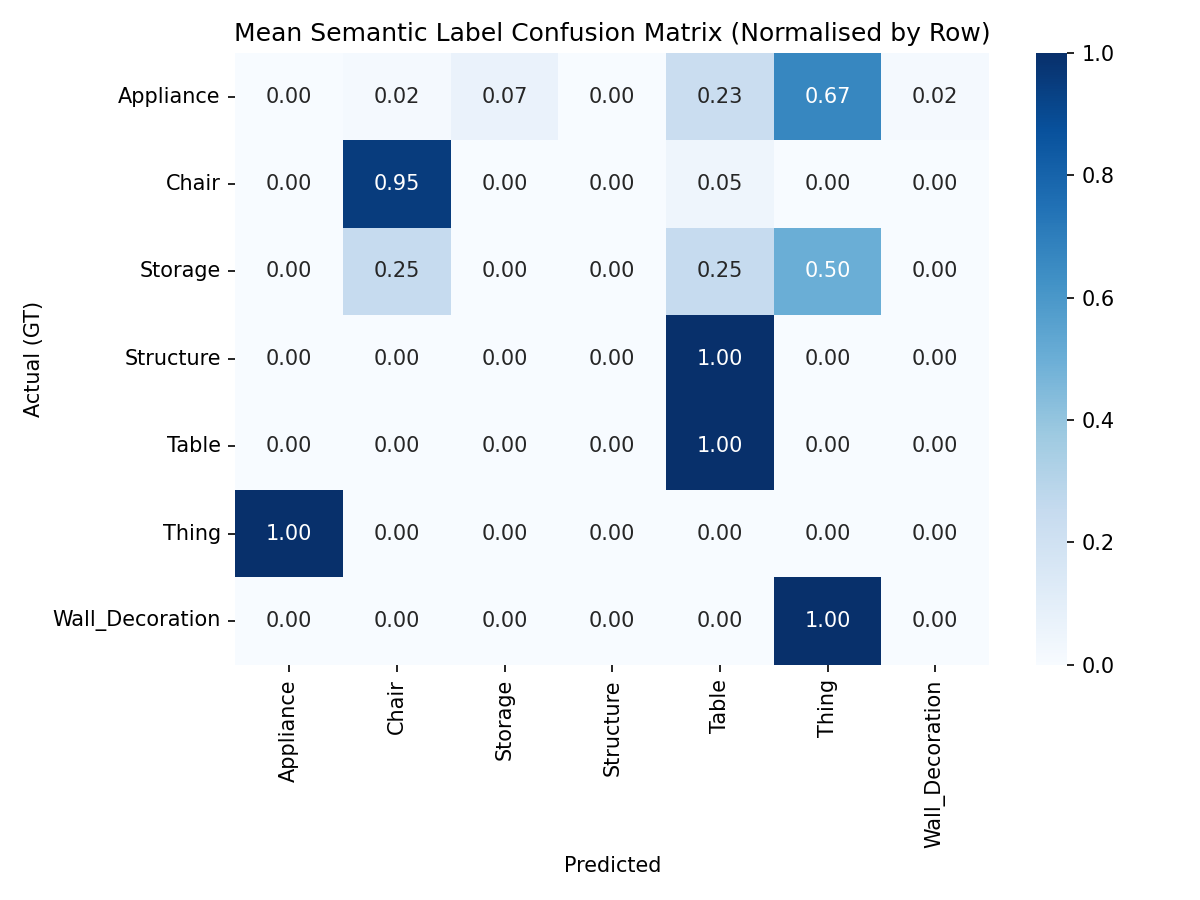
\includegraphics[width=0.5\textwidth]{figures/confusion_matrix_mean_norm.png}
    \caption{Normalised Confusion Matrix of Hydra Labels vs Ground Truth Labels}
    \label{fig:cmatrix}
\end{figure}

\subsection{Practicality}\label{sec:timing}

\begin{table}[H]
\centering
\caption{System Timing Comparison across Stages (Seconds). \textbf{Best results in bold.}}
\label{tab:timing_transposed}
\begin{tabular}{l | ccc | ccc | c}
\toprule
\textbf{Method} & \multicolumn{3}{c|}{\textbf{Frontend}} & \multicolumn{3}{c|}{\textbf{Backend}} & \textbf{Total (Avg)} \\
 & Avg & Std & CV & Avg & Std & CV & \\
\midrule
Hydra    & 0.105 & 0.002 & 0.020 & 0.058 & 0.001 & 0.018 & 0.162 \\
Clio     & \textbf{0.082} & 0.001 & 0.012 & 0.070 & 0.002 & 0.031 & \textbf{0.152} \\
S-Graphs+ & --- & --- & --- & \textbf{0.019} & 0.002 & 0.086 & --- \\
\bottomrule
\end{tabular}
\end{table}

%\lipsum[29-30]

\section{Real-World Results}\label{sec:r-w-results}

\section{Discussion}\label{sec:discussion}
% Critical appraisal: strengths, weaknesses, methodology choices; comparison
% with prior work. Optional: ablation analysis, sensitivity analysis.

%\lipsum[31-32]

\section{Limitations}\label{sec:limitations}
% Limitations, threats to validity, and suggested further tests if not all done.

%\lipsum[33-34]


\chapter{Conclusions and Future Work}\label{ch5}
% =============================================================================
% CHAPTER 5: Conclusions and Future Work
% =============================================================================
% SPDX-FileCopyrightText: 2026 Frank Langbein <frank@langbein.org>
% SPDX-License-Identifier: LPPL-1.3c
%
% Suggested sections: Conclusions; Future work. Do not introduce new material in
% Conclusions---summarise aims and main results. Future work: next steps, open
% questions, what you would do with more time. Optional: short summary of
% contributions (as part of Conclusions or a bullet list).
% =============================================================================

This chapter summarises the main parts of project including the context, objectives. methods , results. Finishing with a discussion of the potential future work for a more in-depth evaluation.

%\lipsum[35-36]

\section{Conclusions}\label{sec:conclusions}
% Summary of aims, key results, and main takeaways. Optional: list of contributions.

The objective of this project was to identify which candidate 3D scene graph method is most suitable for assisting with architectural tasks, such as inventorying or remote building visualisation. Accurate metric data and semantic understanding is important for executing higher-level tasks as the robot needs to know more than what is geometrically around it.

The project consisted of implementing three individual environments capable of deploying the candidate methods justified in \ref{sec:methods}, which consisted of one native and two Docker environments. Each method was then deployed on a custom office dataset, recorded using a differential drive robot with a 3D LiDAR and fixed camera. The results would then allow a complete evaluation of metric and semantic accuracy as well as practicality (detailed metrics outlined in \ref{sec:eval-framework}). These metrics were designed to reveal which method was the most deployment-ready for assisting in architectural tasks.

After analysing the results, it was determined in section \ref{sec:res:best-method} that Hydra was the best-performing method for the architectural industry. This was due to its accuracy and efficiency under hardware constraints, which is likely to be a factor outside of academic institutions.

In comparison, S-Graphs+ was marginally superior at room segmentation, however lacks semantic understanding of the scene. Clio demonstrated strong metric-semantic room segmentation, however it was found to really struggle to instantiate object primitives, likely due to the lack of object frame captures provided by the differential drive and fixed camera used for the dataset. This was contrasted with Hydra which adapted comfortably to the perspective change. As well as this, despite expected behaviour on its example dataset, Clio had to be processed at 0.25 playback speed on the custom office dataset to prevent missing frames or crashing, meaning it was labelled incapable of real-time usage. This nullified Clio as a suitable candidate as it failed one of the mandatory requirements set out in \ref{sec:spec:mandatory}.

There were limitations to this evaluation. Most notably a single environment prevented comparisons over different deployment contexts such as office vs hospital. Another key limitation identified was the data collection method, which limited the coverage and views of objects, likely resulting in the Clio bottleneck observed in section \ref{sec:disc-clio-rec}.

%\lipsum[37-38]

\section{Future work}\label{sec:future}
% Next steps, open questions, and what you would do with more time or resources.

A limitation of this work was an evaluation over one scene context (an office). For a deeper evaluation over different use-cases, the methods could be evaluated over multiple scenes. For example, a warehouse would allow evaluation of detecting different types of boxes, and a hospital scene could demonstrate a humanly dense environment with dynamic parts such as bed curtains etc.

Another key limitation identified was the data collection method. The scene was recorded using a differential drive robot with a fixed camera, which provides a realistic insight into the methods likely available in the architecture world. However, a dataset recorded with a more dynamic robot such as a Reachy2 \cite{Reachy2}, which supports omnidirectional travel as well as a rotatable camera, would allow a larger coverage of the scene and objects which would give the methods more data resulting in more accurate representations.

%\lipsum[39-40]


\chapter{Reflection on Learning}\label{ch6}
% =============================================================================
% CHAPTER 6: Reflection on Learning
% =============================================================================
% SPDX-FileCopyrightText: 2026 Frank Langbein <frank@langbein.org>
% SPDX-License-Identifier: LPPL-1.3c
%
% Suggested sections: Critical narrative of the experience; Analysis and application;
% Implications for future practice. Focus on transferable learning and (where
% applicable) ``double loop learning'': impact on assumptions and concepts, not
% only skills. Optional alternatives: ``What I would do differently''; ``Transferable
% skills and concepts''. Omit this chapter if not required by your institution;
% comment out the \chapter and \input in main.tex.
% =============================================================================

This chapter reflects on what was learned from the project: how assumptions and decisions were re-evaluated and what would be done differently in future.

\section{Critical narrative of the experience}\label{sec:ref:challenges}
% Key challenges, turning points, and how they affected your understanding.

\subsection{Hardware Research}\label{sec:ref:hardware-research}

A key issue during the deployment process was a hardware mismatch when running Hydra. At first, my plan was to deploy the methods on my personal laptop containing a AMD Ryzen 7 5000 Series with AMD Radeon Graphics, this was due to portability and accessibility of a personal laptop compared to a lab desktop. 

I originally deployed each method sequentially: S-Graphs+, Hydra then Clio. Due to S-Graphs+ not needing and specialist hardware, it deployed without issue on my personal laptop. However, when deploying Hydra initially, it would only output the updating frames without constructing or building a graph. 

The cause was identified as a hardware mismatch, as Hydra requires a system capable of running Nvidia TensorRT in order to process frames correctly. This led me to moving to the HCCR lab computer with specs outlined in Table \ref{tab:hardware_specs}, which satisfied this requirement. 

This experience taught me to properly research the ideal hardware specifications before starting deployment.

\subsection{Environment Isolation}\label{sec:ref:environment-isolation}

Another issue was encountered when trying to run all methods on a native environment. S-Graphs+ was originally deployed on ROS2 Humble. As outlined in the Hydra-ROS github \cite{hydra-ros-repo}, Hydra has only been tested on ROS2 Iron and ROS2 Jazzy. 

Due to S-Graphs+ being reported working for ROS2 Iron also, the environment was switched to cater for Hydra compatibility. This caused some issues during integration which created a complex and messy native environment. 

This became more complex later due to Clio still using ROS1 Noetic. After the decision to move to the HCCR lab computer, Dockers were used from the start when deploying Hydra and Clio which made the transition between deploying the methods easier. 

This journey taught me the importance of individual deployment environments when running complex systems.

\subsection{Community Insights}\label{sec:ref:community-insights}

During initial Clio deployment, I used a ROS1 Noetic container which I installed from \cite{shakeri2023docker}. A problem was encountered during Clio installation which kept preventing the catkin build for the Clio workspace. 

This problem was found to be a known issue on a community forum which identified the problem being Clio using ROS1, where many of the main branches of the dependencies had upgraded to ROS2, which caused integration problems. 

A user on the community forum had created and published a Docker container which points directly to the deprecated ROS1 versions for dependencies. This community solution saved the extra work that would be needed to solve each dependency in a new container. This taught me the value of community solutions.



%\lipsum[41-42]

\section{Analysis and application}\label{sec:reflection}
% How you analysed the experience and applied learning to decisions or concepts.

\subsection{Hardware Research}\label{sec:ref:hardware-research-analysis}

This issue has taught me that time should be taken into researching the hardware requirements before the deployment stage begins. I applied this lesson almost immediately as I identified that Clio requires the same TensorRT capability as Hydra. Therefore, in addition to maintaining a fair test with the same hardware, I knew to not even try to deploy it on my personal laptop first, but begin on the lab computer.

\subsection{Environment Isolation}\label{sec:ref:environment-isolation-analysis}

I began this project assuming that different versions of the same system, for example ROS2 releases, often didn’t matter in terms of deployment. However this experience changed this assumption and has taught me that, especially with state-of-the-art systems, even the smallest dependency can cause cascading failures. Like with the hardware, I applied this lesson directly into my Clio deployment by beginning by building a ROS Noetic container to run Clio independently.

\subsection{Community Insights}\label{sec:ref:community-insights-analysis}

This experience taught me the importance of community-driven solutions. As my research led me to valuable resources which saved me considerable time in view of the time constraints of the project. This has highlighted the importance of the open-source community in efficient development processes.

%\lipsum[43-44]

\section{Implications for future practice}\label{sec:implications}
% What you will take forward: habits, assumptions, or approaches in future work.

In the future, I will prioritise creating individual running environments using Docker containers and virtual environments, as this gives me control and stability within systems. As well as this, I will be more mindful of hardware requirements by not prioritising ease-of-use over productivity. I will also incorporate research into community solutions into my development pipelines to ensure I am using my time efficiently by not repeating mistakes someone has already addressed.

%\lipsum[45-46]

\backmatter

% -----------------------------------------------------------------------------
% Appendices
% -----------------------------------------------------------------------------
\appendix
\chapter{Supplementary Material}\label{app:supp}
% =============================================================================
% Appendix: Supplementary Material
% =============================================================================
% SPDX-FileCopyrightText: 2026 Frank Langbein <frank@langbein.org>
% SPDX-License-Identifier: LPPL-1.3c
%
% Appendices hold supporting material (detailed tables, derivations, survey text,
% user-study materials) so the main narrative stays focused. Complete source
% code is usually submitted separately, not in the report. Use \chapter and
% \section as in main chapters. Replace with your own supplementary material.
% =============================================================================

This appendix contains supplementary material like tables containing raw data

\section{Additional tables}\label{app:tables}

\subsection{Label Mapping and Semantics}\label{app:semantics}

\begin{table}[H]
\centering
\caption{Semantic Label Mapping Rules}
\label{tab:label_mapping}
\begin{tabular}{ll | ll}
\toprule
\textbf{Original Label} & \textbf{Mapped Class} & \textbf{Substring Rule} & \textbf{Mapped Class} \\ \midrule
table\_and\_chairs      & Table                 & 'chair'                 & Chair                 \\
office\_chair           & Chair                 & 'computer'              & Appliance             \\
hangout\_chair          & Chair                 & 'whiteboard'            & Wall\_Decoration      \\
office\_box             & Storage               & 'toilet'                & Thing                 \\
mini\_fridge            & Appliance             & 'wastebasket'           & Storage               \\
reception\_desk         & Table                 & 'desk'                  & Table                 \\
corner                  & Structure             & 'monitor'               & Appliance             \\ 
\bottomrule
\end{tabular}
\end{table}


\begin{figure}[H]
    \centering
    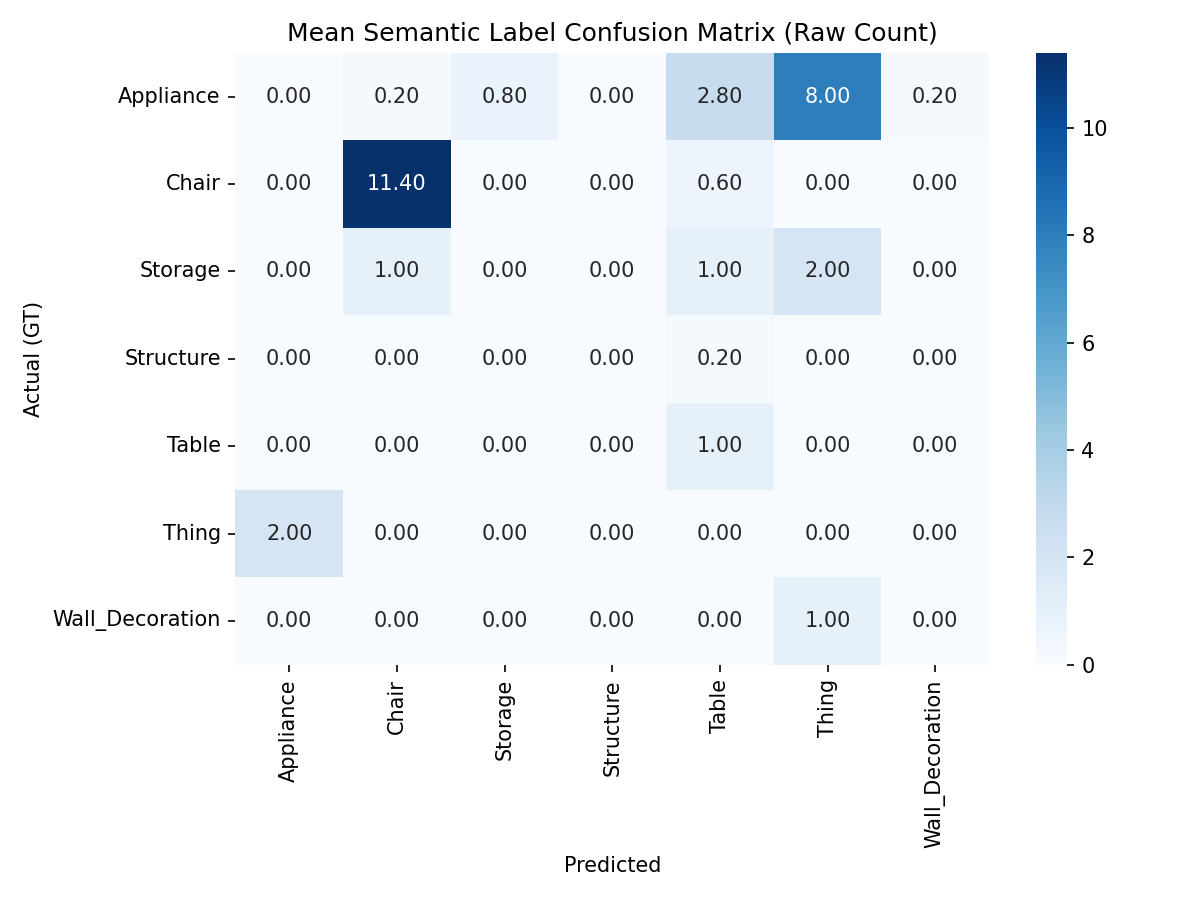
\includegraphics[width=0.9\textwidth]{figures/confusion_matrix_mean_raw.png}
    \caption{Mean Count Confusion Matrix of Hydra Labels vs Ground Truth Labels}
    \label{fig:app:semantics:hydra_cmatrix}
\end{figure}

\subsection{Room Recognition Per-Run}\label{app:room-recognition}

\begin{table}[H]
\centering
\caption{Raw Room Recognition Results over 5 Evaluation Runs}
\label{tab:raw_room_results}
\begin{tabular}{l | ccc | ccc | ccc}
\toprule
\textbf{Run} & \multicolumn{3}{c|}{\textbf{S-Graphs+}} & \multicolumn{3}{c|}{\textbf{Hydra}} & \multicolumn{3}{c}{\textbf{Clio}} \\ 
 & Recall & Precision & F1 & Recall & Precision & F1 & Recall & Precision & F1 \\ \midrule
1 & 0.67 & 0.57 & 0.62 & 0.33 & 1.00 & 0.50 & 1.00 & 0.50 & 0.67 \\
2 & 0.67 & 0.50 & 0.57 & 0.83 & 0.83 & 0.83 & 0.83 & 0.50 & 0.62 \\
3 & 0.67 & 0.57 & 0.62 & 0.50 & 1.00 & 0.67 & 0.83 & 0.42 & 0.56 \\
4 & 0.67 & 0.57 & 0.62 & 0.17 & 1.00 & 0.29 & 1.00 & 0.35 & 0.52 \\
5 & 0.67 & 0.57 & 0.62 & 0.33 & 0.67 & 0.44 & 1.00 & 0.46 & 0.63 \\ \bottomrule
\end{tabular}
\end{table}

\subsection{Object Spatial Accuracy Per-Run}\label{app:spatial-accuracy}

\begin{table}[H]
\centering
\caption{Raw Object Spatial Accuracy (Hydra vs Clio) across 5 Evaluation Runs}
\label{tab:raw_spatial_accuracy}
\begin{tabular}{l | cc | cc}
\toprule
\textbf{Run} & \multicolumn{2}{c|}{\textbf{Hydra}} & \multicolumn{2}{c}{\textbf{Clio}} \\
 & MED (m) & IoU & MED (m) & IoU \\ \midrule
1 & 0.70 & 0.24 & 3.21 & 0.00 \\
2 & 0.73 & 0.23 & 3.51 & 0.00 \\
3 & 0.70 & 0.24 & 3.80 & 0.00 \\
4 & 0.70 & 0.25 & 3.66 & 0.00 \\
5 & 0.74 & 0.23 & 2.63 & 0.00 \\ \bottomrule
\end{tabular}
\end{table}

\begin{table}[H]
\centering
\caption{Detailed Object Drift Statistics (Hydra vs. Clio)}
\label{tab:object_drift_breakdown}
\begin{tabular}{l ccc}
\toprule
\textbf{Label / Category} & \textbf{Mean Drift (m)} & \textbf{Max Drift (m)} & \textbf{Std Dev (m)} \\ \midrule
\textit{Hydra Statistics} & & & \\
Table & 0.14 & 2.56 & 0.35 \\
Chair & 0.07 & 1.62 & 0.23 \\
Thing & 0.09 & 3.14 & 0.40 \\
Couch & 0.05 & 0.05 & 0.00 \\
Door & 0.01 & 0.01 & 0.00 \\
Shelf & 0.21 & 1.52 & 0.47 \\
Plant & 1.46 & 6.69 & 2.72 \\
Appliance & 0.01 & 0.02 & 0.01 \\
Light & 0.06 & 0.12 & 0.03 \\
Storage & 0.18 & 2.59 & 0.57 \\
Wall\_Decoration & 0.03 & 0.09 & 0.02 \\ \midrule
\textbf{Hydra Overall} & \textbf{0.16} & \textbf{6.69} & \textbf{0.72} \\ \midrule
\textit{Clio Statistics} & & & \\
Unknown & 2.18 & 9.22 & 2.74 \\ \midrule
\textbf{Clio Overall} & \textbf{2.18} & \textbf{9.22} & \textbf{2.74} \\ \bottomrule
\end{tabular}
\end{table}


\subsection{Execution Timings Raw Data}\label{app:timings}

\begin{table}[H]
\centering
\caption{Raw Execution Timings across 5 Evaluation Runs (Seconds)}
\label{tab:raw_timings_final}
\resizebox{\textwidth}{!}{
\begin{tabular}{l | cccc | cccc | cc}
\toprule
\textbf{Run} & \multicolumn{4}{c|}{\textbf{Hydra}} & \multicolumn{4}{c|}{\textbf{Clio}} & \multicolumn{2}{c}{\textbf{S-Graphs+ (Backend)}} \\
 & F\_Mean & F\_Max & B\_Mean & B\_Max & F\_Mean & F\_Max & B\_Mean & B\_Max & Mean & Max \\ \midrule
1 & 0.104 & 0.185 & 0.056 & 0.154 & 0.083 & 0.399 & 0.072 & 0.203 & 0.0193 & 0.056 \\
2 & 0.102 & 0.200 & 0.057 & 0.187 & 0.083 & 0.264 & 0.070 & 0.202 & 0.0186 & 0.044 \\
3 & 0.104 & 0.207 & 0.058 & 0.162 & 0.083 & 0.313 & 0.072 & 0.231 & 0.0208 & 0.056 \\
4 & 0.106 & 0.217 & 0.059 & 0.184 & 0.081 & 0.346 & 0.067 & 0.181 & 0.0167 & 0.047 \\
5 & 0.107 & 0.239 & 0.059 & 0.210 & 0.081 & 0.329 & 0.071 & 0.207 & 0.0205 & 0.063 \\ \bottomrule
\end{tabular}
}
\end{table}




%\lipsum[47-48]

% \section{Further analysis}\label{app:analysis}

%\lipsum[49-50]

% \section{Derivation}\label{app:derivation}

%\lipsum[51-52]


% \chapter{Additional Results}\label{app:results}
% \input{AB/appendixB}

% Bibliography (always last): \bib{bibfile} uses natbib (numeric or harvard per class option)
% and inserts the License chapter if \license was set.
\bib{bibliography}

\end{document}
